\begin{tikzpicture}[>=stealth, scale=0.008\columnwidth]
%  \begin{scope}[yshift=1cm]
%    \node (text1) at (0.5,0) {$\Theta: [0,1]^2\newarrow[0,1] \text{ measurable and symmetric}$};
%    \node (text2) at ($(text1)+(3,0)$) {$U_1,U_2,\ldots\simiid\Uniform[0,1]$};
%    \node (text3) at ($(text1)+(1.3,-0.3)$) {$\mbox{Pr}\lbrace \text{edge } i,j\rbrace=\Theta(U_i,U_j)$};
%  \end{scope}
  %% \begin{scope}[yshift=1cm]
  %%   \node (text1) at (1.7,0) {$\Theta: [0,1]^2\newarrow[0,1] \text{ measurable and symmetric}$};
  %%   \node (text2) at ($(text1)+(0,-0.3)$) {$U_1,U_2,\ldots\simiid\Uniform[0,1]$};
  %% \end{scope}
  \begin{scope}[yshift=0cm,xshift=0cm,scale=1.1]
  \begin{scope}
    \path[use as bounding box] (-0.5,0.5) rectangle (2.8,-1.5);
    \draw (0,0) --(0,-1) --(1,-1) --(1,0) --(0,0);
    %\draw (0,0)--(1,-1);
    \node[font=\normalsize] at (0,0.1) {$0$};
    \node[font=\normalsize] at (-0.1,0) {$0$};
    \node[font=\normalsize] at (1,-1.1) {$1$};
    \node[font=\normalsize] at (1.1,-1) {$1$};
    \draw [dashed] (0.2,0.1) -- (0.2,-1.1); \node at (0.2,0.2) {$U_i$};
    \draw [dashed] (-0.1,-0.2) -- (1.1,-0.2); \node at (-0.25,-0.2) {$U_i$};
    \draw [dashed] (0.65,0.1) -- (0.65,-1.1); \node at (0.65,0.2) {$U_j$};
    \draw [dashed] (-0.1,-0.65) -- (1.1,-0.65); \node at (-0.25,-0.65) {$U_j$};
    \node[circle,fill,scale=0.4,color=red] (red1) at (0.65,-0.2) {};
  \end{scope}
  \begin{scope}[yshift=-1.8cm]
    \draw (0,0)--(1,0);
    \draw (0,-0.05)--(0,0.05); \node at (0,-0.15) {$0$};
    \draw (1,-0.05)--(1,0.05); \node at (1,-0.15) {$1$};
    \node[circle,fill,scale=0.4,color=red] (red2) at (0.21,0) {};
    %\node[font=\scriptsize] at (0.48,-0.1) {$\mbox{Pr}\lbrace X_{ij}=1\rbrace=\Theta(U_i,U_j)$};
    \node[font=\large,color=camdarkblue] (flipprob) at (0.21,-0.3) {$\mbox{Pr}\lbrace\text{edge } i,j\rbrace$};
    \draw[->,color=blue!30!gray] ($(flipprob.north)+(0,0)$)--($(red2.south)+(0,-0.03)$);
  \end{scope}
  \begin{scope}
  \draw[->] ($(red1.south east)+(0.01,-0.01)$) .. controls (1,-0.8) and (1,-1.2) .. ($(red2.north east)+(0.01,0.01)$);
  \draw (0.5,-1.4) node [fill=none] {$\Theta$};
  \end{scope}
   \end{scope}
  \begin{scope}[xshift=2.2cm,yshift=-0.55cm]
    \node [mybox] (box1){
  
\includegraphics[width=0.26\columnwidth]{../misc/min_function.pdf} 
 %  \includegraphics[width=2.9cm]{include/uniform_attachment_graphon.pdf}
  };
    \node at ($(box1)+(0.7,0)$) {$\Theta$};
  \end{scope}  
  \begin{scope}[xshift=2.2cm,yshift=-1.8cm]
    \node [mybox] (box2){
      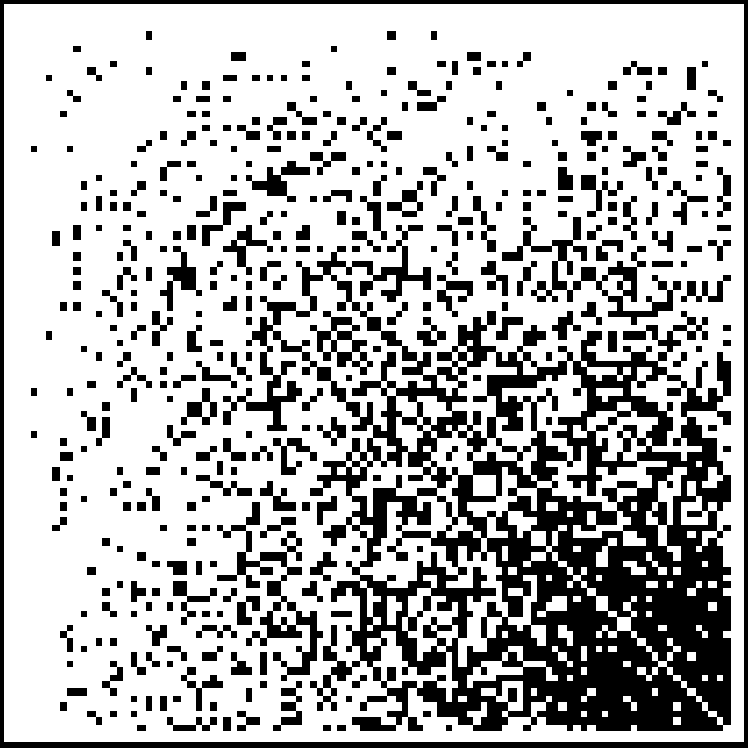
\includegraphics[width=0.26\columnwidth]{../misc/lovasz_sample100.pdf}
%    \includegraphics[width=2.8cm]{include/uniform_attachment_empirical.pdf}
    
  };
\node at ($(box2)+(0.84,0)$) {Sample};
  \end{scope}
\end{tikzpicture}
